\documentclass[a4paper,12pt]{article}

% коментарии к каждому включенному ниже пакету
\usepackage[russian]{babel} % пакет для подготовки текста на русском языке
\usepackage{hyperref} % пакет для генерации ссылок в pdf
\usepackage{geometry} % пакет, который определяет поля страницы
\usepackage{graphicx} % для вставки картинок
\usepackage{verbatim} % для вставки листингов с кодом

% установка геометрии
\geometry{top=2cm, bottom=2cm, left=3cm, right=1.5cm}


\begin{document}

% Титульный лист
\begin{titlepage}
\begin{center}
{\large\scshape\bfseries
министерство науки и высшего образования российской федерации\\
федеральное государственное автономное образовательное учреждение высшего образования\\
«северо-кавказский федеральный университет»\\
факультет математики и компьютерных наук имени профессора н.и.червякова}
\vfill
\Large{\textbf{ЛАБОРАТОРНАЯ РАБОТА №17}}\\[2mm]
\large{Алгоритмизация и программирование}\\[6mm]
\Large{\textbf{Вариант 9}}\\[20mm]
\end{center}
\begin{flushright}
\textbf{Выполнил студент:}\\
Сивко Иван Андреевич\\
студент 2 курса\\
группа ПМИ-б-о-23-2,\\
направление подготовки 01.03.02\\[5mm]
\textbf{Проверил:}\\
Ассистент кафедры вычислительной\\
математики и кибернетики, к.ф.-м.н.,\\
Черкашина Анастасия Андреевна
\end{flushright}
\vfill
\centerline{ \the\year\ г. }
\end{titlepage}


% Основная часть
\centerline{\large\textbf{Вариант 9}}
\textbf{Цель:}
\begin{small}
\begin{itemize}
\item Совершенствование навыков разработки программ в среде программирования
\item Совершенствование навыков в программировании с использованием указателей
\item Исследование процесса формирования элементов простейшей динамической структуры данных – двоичное дерево
\item Исследование операций при работе с двоичными деревьями
\end{itemize}
\end{small}

\section*{Задание 1}
\textit{В соответствии с вариантом напиисать и отладить программу, исполльзуя
динамичискую структуру двнных: Двоичное деревья.}
\renewcommand{\thesubsection}{\arabic{subsection}} % Задания нумерации для \subsection
\setcounter{subsection}{0} % подпункты с 1
\subsection{Условие}
Разработать программу, которая строит двоичное дерево T. Описать процедуру, заменяющую в деереве T все отрицательные элемнты
на их абсалютнве значения.
\subsection{Алгоритм / Математическая модель}

Программа предназначена для работы с бинарным деревом поиска (Binary Search Tree, BST) и выполняет операции добавления, отображения и модификации данных. Алгоритм выполнения программы следующий:

\begin{enumerate}
\item \textbf{Ввод чисел:}
\begin{itemize}
\item Пользователь вводит целые числа построчно.
\item Ввод завершается пустой строкой.
\item Числа добавляются в бинарное дерево поиска.
\end{itemize}

\item \textbf{Печать дерева:}
\begin{itemize}
\item Дерево выводится на экран в упорядоченном (in-order) порядке.
\item Если дерево пустое, вывод на экран не выполняется.
\end{itemize}

\item \textbf{Замена отрицательных значений:}
\begin{itemize}
\item В каждом узле дерева отрицательные значения заменяются их модулями.
\end{itemize}

\item \textbf{Повторная печать дерева:}
\begin{itemize}
\item После преобразования дерево снова выводится в упорядоченном виде.
\end{itemize}

\item \textbf{Выход:} Программа завершает свою работу.
\end{enumerate}

\subsubsection{Математическая модель}
\textbf{Бинарное дерево поиска (BST):} Дерево представлено как тройка:
\[ T = (N, L, R) \]
где \(N\) — значение узла, \(L\) — левое поддерево, \(R\) — правое поддерево. Для любого узла выполняется:
\[ \forall x \in L, \; x < N; \quad \forall y \in R, \; y \geq N. \]
\subsection{Диаграмма:}
\begin{figure}[h]
\centering
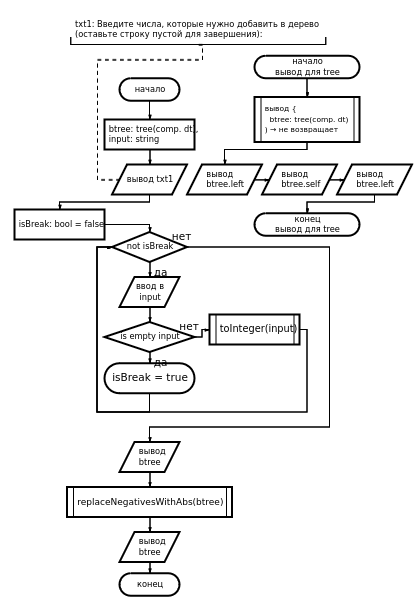
\includegraphics[width=0.8\textwidth]{data/diagram17.png}
\end{figure}
\subsection{Код:}
\verbatiminput{data/task17.cpp}
\href{https://raw.githubusercontent.com/John1400800/stuff/refs/heads/main/c_learning/home_works/task17.cpp}{source code}
\subsection{Результат работы программы:}
\begin{figure}[h]
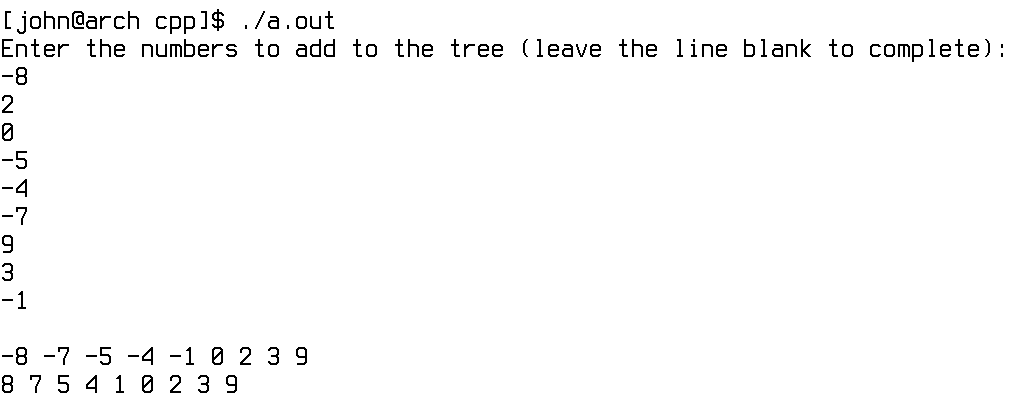
\includegraphics[width=0.8\textwidth]{data/demo17.png}
\end{figure}
\end{document}
